% Lecture Template (handout) for ME3001 - Mechanical Engineering Analysis - Tennessee Technological University
% Spring 2024 - condensing and streamlining lectures by combining topics into a single PDF under the module name
% this will simplify file and link management as well as make lectures easier to use in class
% - added image/ to clean directory and reduce redundancy, specific to module for now  

% Module Name: - Non-Linear Equations
% Topic 1 - Solving Non-Linear Equations
% Topic 2 - The Newton-Raphson Method, Secant Method
% Topic 3 - The Bisection Method
% Topic 4 - Mechanical Design Problem

\documentclass[fleqn]{beamer} % for presentation (has nav buttons at bottom)

\usepackage{../analysis_lectures}

\author{ME3001 - Mechanical Engineering Analysis}

\newcommand{\MNUM}{2\hspace{2mm}} % module number 
\newcommand{\moduletitle}{Non-Linear Equations}

\newcommand{\sectionItitle}{Solving Non-Linear Equations}
\newcommand{\sectionIItitle}{The Newton-Raphson Method, Secant Method}
\newcommand{\sectionIIItitle}{The Bisection Method}
\newcommand{\sectionIVtitle}{Mechanical Design Problem}

\newcommand{\sectionIsubsectionItitle}{What is a Non-Linear Equation ?}
\newcommand{\sectionIsubsectionIItitle}{Solving Non-linear Equations}
\newcommand{\sectionIsubsectionIIItitle}{Analytical vs. Numerical Methods}
\newcommand{\sectionIsubsectionIVtitle}{Example}

\newcommand{\sectionIIsubsectionItitle}{Classification of Methods}
\newcommand{\sectionIIsubsectionIItitle}{Taylor Series Derivation}
\newcommand{\sectionIIsubsectionIIItitle}{The Newton Raphson Method}
\newcommand{\sectionIIsubsectionIVtitle}{The Finite Difference}
\newcommand{\sectionIIsubsectionVtitle}{Modified Newton-Raphson, Secant Method}
\newcommand{\sectionIIsubsectionVItitle}{Algorithm Comparison}

\newcommand{\sectionIIIsubsectionItitle}{Analytical vs. Numerical}
\newcommand{\sectionIIIsubsectionIItitle}{A Bracketing Method: Graphical Explanation}
\newcommand{\sectionIIIsubsectionIIItitle}{Algorithm Description}
\newcommand{\sectionIIIsubsectionIVtitle}{Programming Exercise}

\newcommand{\sectionIVsubsectionItitle}{Problem Statement}
\newcommand{\sectionIVsubsectionIItitle}{Mathematical Model}
\newcommand{\sectionIVsubsectionIIItitle}{Solution Approach}
\newcommand{\sectionIVsubsectionIVtitle}{Design}

% custom box
\newsavebox{\mybox}

\title{Lecture Module - \moduletitle}

\date{Mechanical Engineering\vspc Tennessee Technological University}

\begin{document}

	\lstset{language=MATLAB,basicstyle=\ttfamily\small,showstringspaces=false}

	\frame{\titlepage \center\begin{framed}\Large \textbf{Module \MNUM - \moduletitle}\end{framed} \vspace{5mm}}

	% Module Outline
	\begin{frame} 
		\large \textbf{Module \MNUM - \moduletitle} \vspace{3mm}\\

		\begin{itemize}
			\item Topic 1 - \hyperlink{sectionI}{\sectionItitle} \vspc % section I
			\item Topic 2 - \hyperlink{sectionII}{\sectionIItitle} \vspc % section II
			\item Topic 3 - \hyperlink{sectionIII}{\sectionIIItitle} \vspc % section III
		\end{itemize}

	\end{frame}

	% section I
	\section{\sectionItitle}\label{sectionI}

		% section I Outline
		\begin{frame} 
			\large \textbf{Topic 1 - \sectionItitle} \vspace{3mm}\\

			\begin{itemize}
				\item \hyperlink{sectionIsubsectionI}{\sectionIsubsectionItitle} \vspc %  section I subsection I
				\item \hyperlink{sectionIsubsectionII}{\sectionIsubsectionIItitle} \vspc % section I subsection II
				\item \hyperlink{sectionIsubsectionIII}{\sectionIsubsectionIIItitle} \vspc % section I subsection III
				\item \hyperlink{sectionIsubsectionIV}{\sectionIsubsectionIVtitle} \vspc % section I subsection IV
			\end{itemize}
		\end{frame}
		
		% section I subsection I 
		\subsection{\sectionIsubsectionItitle}\label{sectionIsubsectionI}

			\begin{frame}
				\frametitle{\sectionIsubsectionItitle}
				\bigskip

				\textbf{Different Types of Non-Linear Equations }
		
				\begin{itemize}
					\item \textbf{Polynomials (excluding first order)} \vspace{3mm}
					\item \textbf{ Transcendentals} \vspace{2mm}

					{" a transcendental function "transcends" algebra in that it cannot be expressed in terms of a finite sequence of the algebraic operations of addition, multiplication, and root extraction. Examples of transcendental functions include the exponential function, the logarithm, and the trigonometric functions. "}\\
					\begin{itemize}
						\item Exponentials \vspace{1mm}
						\item Logarithms \vspace{1mm}
						\item Trigonometrics \vspace{2mm}
					\end{itemize}

				\end{itemize}

				\btVFill
			\end{frame}

			\begin{frame}
				\frametitle{\sectionIsubsectionItitle}
				\bigskip

				\btVFill
			\end{frame}

		% section I subsection II
		\subsection{\sectionIsubsectionIItitle}\label{sectionIsubsectionII}

			\begin{frame}
				\frametitle{\sectionIsubsectionIItitle}
				\bigskip

					\textbf{ Example:} Solve the following equation. \vspace{2mm} \\

					\hspace{2mm}\scalebox{1.0}{$y = x^2 + 2x - 10$}	 \vspace{2mm}

					\hspace*{-1cm}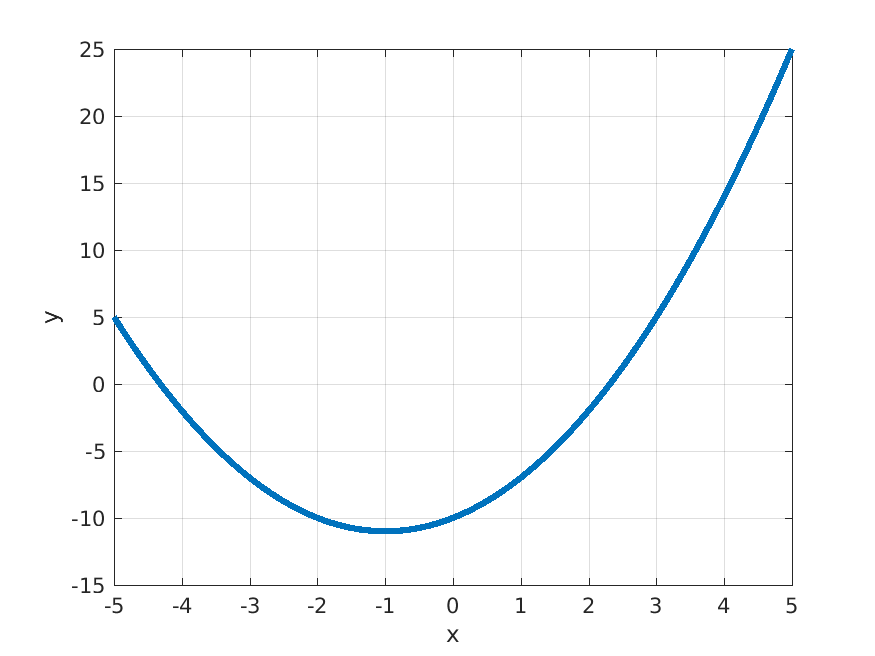
\includegraphics[scale=.45]{images/lecture1_fig1.png}  

				\btVFill
			\end{frame}

				%\btVFill
			\begin{frame}
				\frametitle{\sectionIsubsectionIItitle}
				\bigskip

				Defintion of \textbf{Solution} 
				\begin{itemize}
					\item - \vspccc
					\item - \vspccc
					\item - \vspccc
				\end{itemize}

				\btVFill
			\end{frame}

		% section I subsection III
		\subsection{\sectionIsubsectionIIItitle}\label{sectionIsubsectionIII}
			\begin{frame} 
				\frametitle{\sectionIsubsectionIIItitle}
				\bigskip

				\textbf{Analytical}
				\begin{itemize}
					\item solution to a problem that can be written in {\bf closed form} 
					\item solution in terms of known functions, constants, etc.  
					\item gives an {\bf exact answer}  \vspcc
				\end{itemize}

				\textbf{Numerical}
				\begin{itemize}
					\item an {\bf approximation} to the solution of a mathematical equation
					\item iterative procedure or algorithm
					\item 
				\end{itemize}

				\btVFill
			\end{frame}	

		% section I subsection IV
		\subsection{\sectionIsubsectionIVtitle}\label{sectionIsubsectionIV}	

			\begin{frame}
				\frametitle{\sectionIsubsectionIVtitle}
				\bigskip

				We are looking for where the line crosses the x-axis, so how can we tell where this happens? \vspace{1mm}\\

				\begin{multicols}{2}
				\scalebox{1.0}{$y = x^2 + 2x - 10$} \vspace{3mm}\\

				\hspace*{-1cm}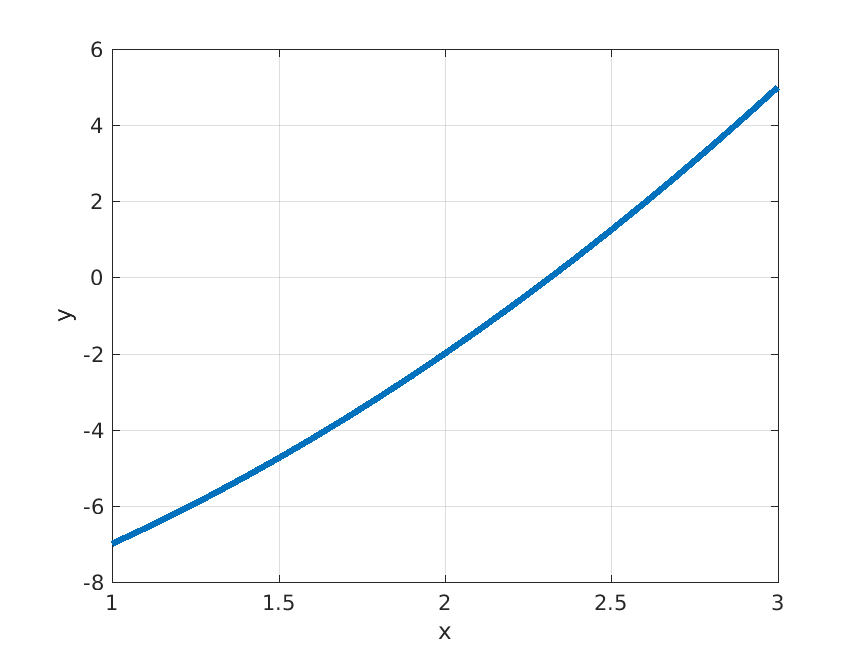
\includegraphics[scale=.4]{images/lecture1_fig3.png}
				\end{multicols}

				\btVFill
			\end{frame}
	
	% Section II
	\section{\sectionIItitle}\label{sectionII}

		% section II Outline
		\begin{frame}
			\large \textbf{Topic 2 - \sectionIItitle} \vspace{3mm}\\

			\begin{itemize}
				\item \hyperlink{sectionIIsubsectionI}{\sectionIIsubsectionItitle} \vspc %  section II subsection I
				\item \hyperlink{sectionIIsubsectionII}{\sectionIIsubsectionIItitle} \vspc % section II subsection II
				\item \hyperlink{sectionIIsubsectionIII}{\sectionIIsubsectionIIItitle} \vspc % section II subsection III
				\item \hyperlink{sectionIIsubsectionIV}{\sectionIIsubsectionIVtitle} \vspc % section II subsection IV
				\item \hyperlink{sectionIIsubsectionV}{\sectionIIsubsectionVtitle} \vspc % section II subsection V
				\item \hyperlink{sectionIIsubsectionVI}{\sectionIIsubsectionVItitle} \vspc % section II subsection VI
			\end{itemize}

		\end{frame}

		% section II subsection I
		\subsection{\sectionIIsubsectionItitle}\label{sectionIIsubsectionI}

			\begin{frame}[label=sectionIIsubsectionI]
				\frametitle{\sectionIIsubsectionItitle}
				\bigskip

				\vspace{5mm}  	
				\textbf{ Theoretical/Analytical Solution Techniques }
				\begin{itemize}
					\item solving the equation using exact mathematics \\
					\item leads to an exact or {\it analytical} solution \\ 	\vspace{10mm}
				\end{itemize}
				\textbf{ Numerical Solution Techniques }		
				\begin{itemize}
					\item  approximating the solution to the equation using varying methods, or {\it algorithms}  \\
					\item leads to a approximate solution \\ 
					\item a.k.a. {\it Numerical Method}\vspace{20mm}
				\end{itemize}

				\btVFill
			\end{frame}

			\begin{frame}[label=sectionIIsubsectionI]
				\frametitle{\sectionIIsubsectionItitle}
				\bigskip

				These scientists changed the world forever.

				\begin{itemize}
					\item Isaac Newton, mathematician and physicist, 1642-1727
					\item Joseph Raphson, English Mathematician, 1648-1715 \\
					\item add Taylor to list \\
				\end{itemize}

				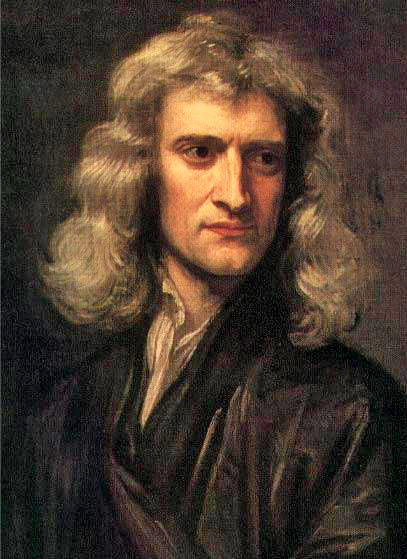
\includegraphics[scale=.17]{images/newton_portrait.jpg}
				\hspace{10mm}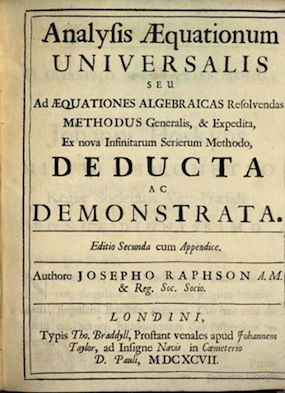
\includegraphics[scale=.30]{images/raphson_book.jpg}

				\btVFill
			\end{frame}	

			\begin{frame}[label=sectionIIsubsectionI]
				\frametitle{\sectionIIsubsectionItitle}
				\bigskip

				The Newton-Raphson method is a {\it shooting method}. \vspace{5mm}

				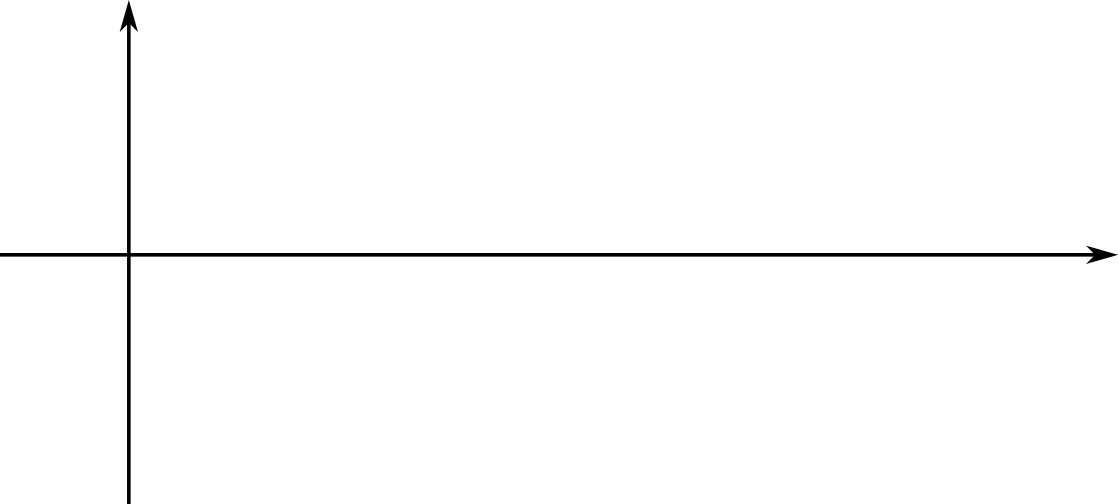
\includegraphics[scale=.40]{images/topic3_fig1.png}
				
				\btVFill
			\end{frame}

		% section II subsection II
		\subsection{\sectionIIsubsectionIItitle}\label{sectionIIsubsectionII}

			\begin{frame}
				\frametitle{\sectionIIsubsectionIItitle}
				\bigskip

				The method can be derived from the Taylor series. \vspace{5mm} \\
	
				\scalebox{1}{$f(x)\approx f(a)+f'(a)(x-a)+\frac{f''(a)}{2!}(x-a)^2+...+\frac{f^{(n)}(a)}{n!}(x-a)^{(n)}$} \vspace{50mm}
		
				\btVFill 
			\end{frame}	

			\begin{frame}
				\frametitle{\sectionIIsubsectionIItitle} \small
				\bigskip

				The 4 possible sign (+/-) cases are handled by the algorithm. 

				Now you have much better hammer. However, must be used properly... \vspace{3mm}\\
				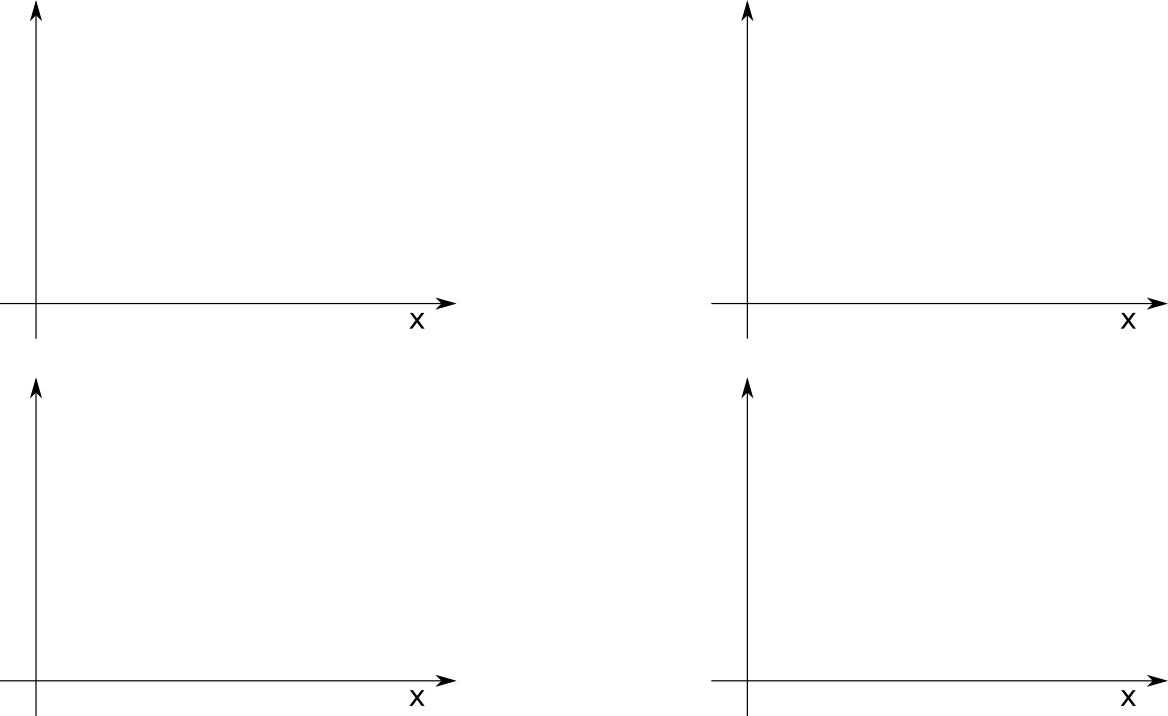
\includegraphics[scale=.35]{images/topic3_fig2.png}

				\btVFill
			\end{frame}		


		% section II subsection III
		\subsection{\sectionIIsubsectionIIItitle}\label{sectionIIsubsectionIII}

			\begin{frame}
				\frametitle{\sectionIIsubsectionIIItitle}
				\bigskip

				\textbf{Algorithm Summary:}
				\begin{itemize}
					\item - Step 1: start doing stuff 
					\item - Step 2: do more stuff
					\item - Step 3: keep doing stuff until you have the solution
				\end{itemize}
				\btVFill 
			\end{frame}

			\begin{frame}
				\frametitle{\sectionIIsubsectionIIItitle}\small
				\bigskip

				\textbf{General Use Algorithm:} a much better hammer ...\vspcc

				\underline{Pros:}
				\begin{itemize}
			    	\item can be used for many different equations
			    	\item problem specific algebra not required to obtain value of solution 
			    	\item executiion of numerical method is routine and can automated
				\end{itemize} 

				\underline{Cons:}
				\begin{itemize}
					\item problem definition can be the difficult
					\item solution results and computation time dependent on initial estimation 
					\item numerical solution must be computed for with defined equation parameters
				\end{itemize}

				\btVFill 
			\end{frame}

			\begin{frame}
				\frametitle{\sectionIIsubsectionIIItitle} \scriptsize
				\bigskip
				
				\textbf{4 General Use Cases}
				\begin{itemize}
					\item The general problem of solving for the root of a non linear equation can be extended to 4 useful 
					variants. 
					\item With careful equation setup, all cases can be solved with the same systematic routine. 	
				\end{itemize}	
				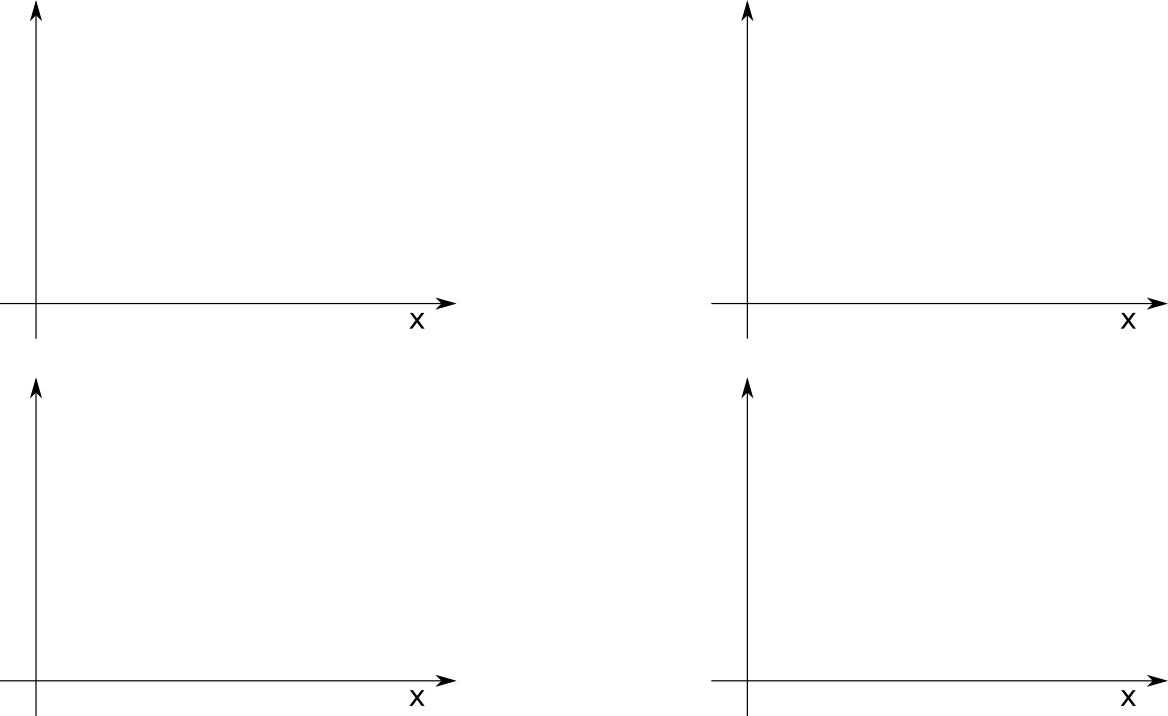
\includegraphics[scale=.3]{images/topic3_fig2.png}			
			
				\btVFill 
			\end{frame}

			\begin{frame}
				\frametitle{\sectionIIsubsectionIIItitle}
				\bigskip

				\btVFill 
			\end{frame}

		% section II subsection IV 
		\subsection{\sectionIIsubsectionIVtitle}\label{sectionIIsubsectionIV}

			\begin{frame}
				\frametitle{\sectionIIsubsectionIVtitle}
				\bigskip

				Our goal is to write a computer program to automate the Newton-Raphson method. We want our program to be (1) robust to different inputs and (2) user friendly. 

				\btVFill 
			\end{frame}

			\begin{frame}
				\frametitle{\sectionIIsubsectionIVtitle}
				\bigskip

				\textbf{The Newton-Raphson method is not \PR{purely numerical}\BK, why?} \\
				\begin{itemize}
					\item  The Equation\vspace{3mm}	\\
					\item  The Derivation\vspace{3mm}	\\
				\end{itemize}
				\textbf{How can we avoid this issue?} \vspace{10mm}\\

				\textbf{{\it Hint:} Think about the title \PR{secant} \BK ...} \vspace{10mm}\\

				\btVFill 
			\end{frame}

			\begin{frame}
				\frametitle{\sectionIIsubsectionIVtitle}
				\bigskip

				This idea or technique is the foundation of a family of methods known as the {\it \PN Finite Difference Methods}.

				\begin{multicols}{3}

					Forward\\
					Difference\\
					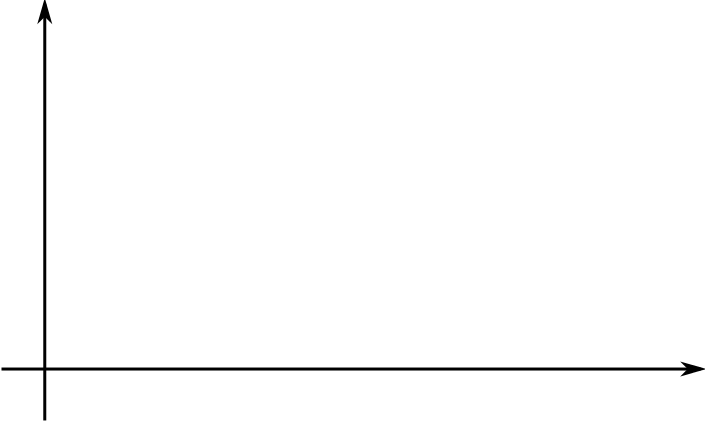
\includegraphics[scale=.14]{images/lecture4_fig1.png}\\

					Backwards\\
					Difference\\
					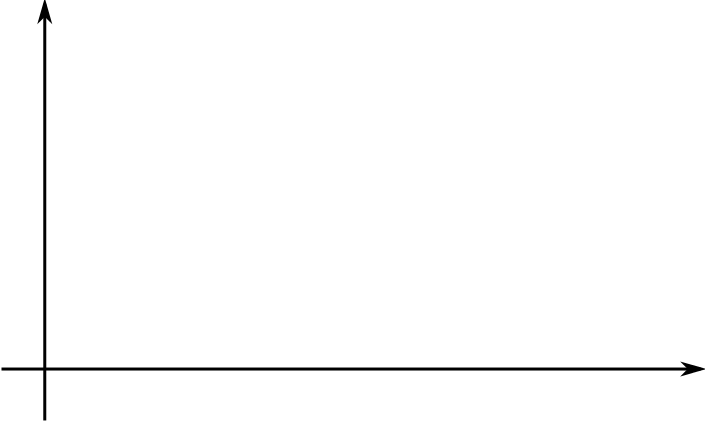
\includegraphics[scale=.14]{images/lecture4_fig1.png}\\

					Central\\
					Difference\\
					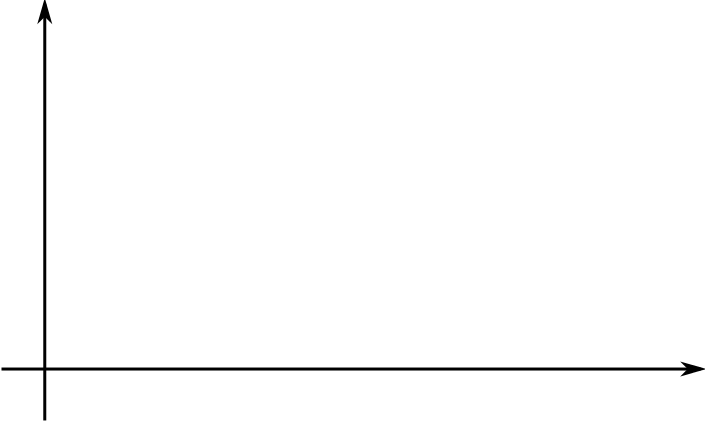
\includegraphics[scale=.14]{images/lecture4_fig1.png}\\
				
				\end{multicols}

				\btVFill 
			\end{frame}

		% section II subsection V 
		\subsection{\sectionIIsubsectionVtitle}\label{sectionIIsubsectionV}

			\begin{frame}
				\frametitle{\sectionIIsubsectionVtitle}
				\bigskip

				The {\PR secant} method is a modified version of the Newton-Raphson method which uses the Finite difference method to compute the slope values of the function to be solved. \\

				\begin{multicols}{2}
				Newton-Raphson
				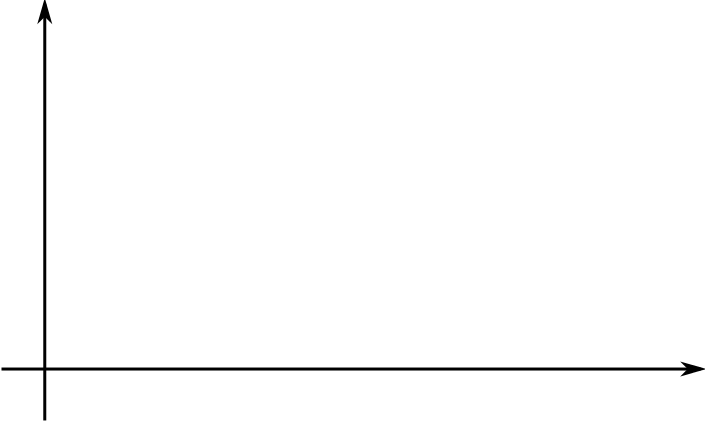
\includegraphics[scale=.22]{images/lecture4_fig1.png} 
				Secant
				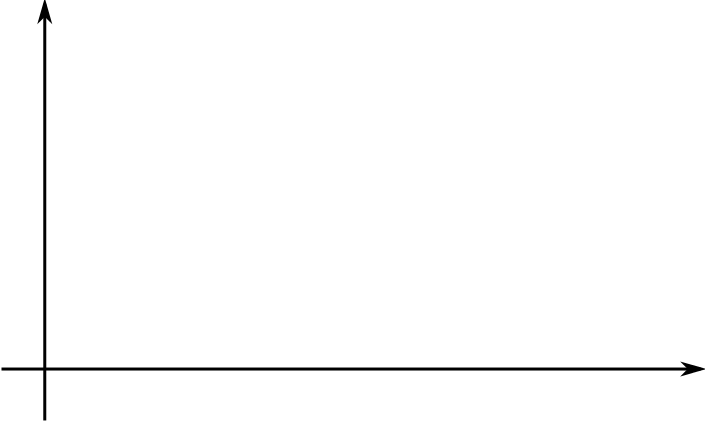
\includegraphics[scale=.22]{images/lecture4_fig1.png}
				\end{multicols}

			
				\btVFill 
			\end{frame}

			\begin{frame}
				\frametitle{\sectionIIsubsectionVtitle}
				\bigskip

				\textbf{Algorithm Summary:}
				\begin{itemize}
					\item - Step 1: start doing stuff 
					\item - Step 2: do more stuff
					\item - Step 3: keep doing stuff until you have the solution
				\end{itemize}
				\btVFill 
			\end{frame}

			\begin{frame}
				\frametitle{\sectionIIsubsectionVtitle}\small
				\bigskip

				\textbf{General Use Algorithm:} the secant method is a generalized, numerical tool for solving non linear equations \vspcc
				\underline{Pros:}
				\begin{itemize}
			    	\item -
			    	\item -
			    	\item -
				\end{itemize} 

				\underline{Cons:}
				\begin{itemize}
					\item -
					\item -
					\item -
				\end{itemize}
				
				\btVFill 
			\end{frame}	
		
	% Section III
	\section{\sectionIIItitle}\label{sectionIII}

		% section III Outline
		\begin{frame}
			\large \textbf{Topic 3 - \sectionIIItitle} \vspace{3mm}\\

			\begin{itemize}
				\item \hyperlink{sectionIIIsubsectionI}{\sectionIIIsubsectionItitle} \vspc %  section III subsection I
				\item \hyperlink{sectionIIIsubsectionII}{\sectionIIIsubsectionIItitle} \vspc % section III subsection II
				\item \hyperlink{sectionIIIsubsectionIII}{\sectionIIIsubsectionIIItitle} \vspc % section III subsection III
				%\item \hyperlink{sectionIIIsubsectionIV}{\sectionIIIsubsectionIVtitle} \vspc % section III subsection IV
			\end{itemize}

		\end{frame}

		% section III subsection I
		\subsection{\sectionIIIsubsectionItitle}\label{sectionIIIsubsectionI}

			\begin{frame}
				\frametitle{\sectionIIIsubsectionItitle}
				\bigskip

				\vspace{5mm}  	
				\textbf{ Theoretical/Analytical Solution Techniques }
				\begin{itemize}
					\item solving the equation using exact mathematics \\
					\item leads to an exact or {\it analytical} solution \\ 	\vspace{10mm}
				\end{itemize}
				\textbf{ Numerical Solution Techniques }		
				\begin{itemize}
					\item  approximating the solution to the equation using varying methods, or {\it algorithms}  \\
					\item leads to a approximate solution \\ 
					\item a.k.a. {\it Numerical Method}\vspace{20mm}
				\end{itemize}
					
				\btVFill
			\end{frame}

			\begin{frame}
				\frametitle{\sectionIIIsubsectionItitle}
				\bigskip

				\btVFill
			\end{frame}

		% section III subsection II
		\subsection{\sectionIIIsubsectionIItitle}\label{sectionIIIsubsectionII}	

			\begin{frame}
				\frametitle{\sectionIIIsubsectionIItitle}
				\bigskip

				The Bisection method is a {\it bracketing method}. \vspace{5mm}
				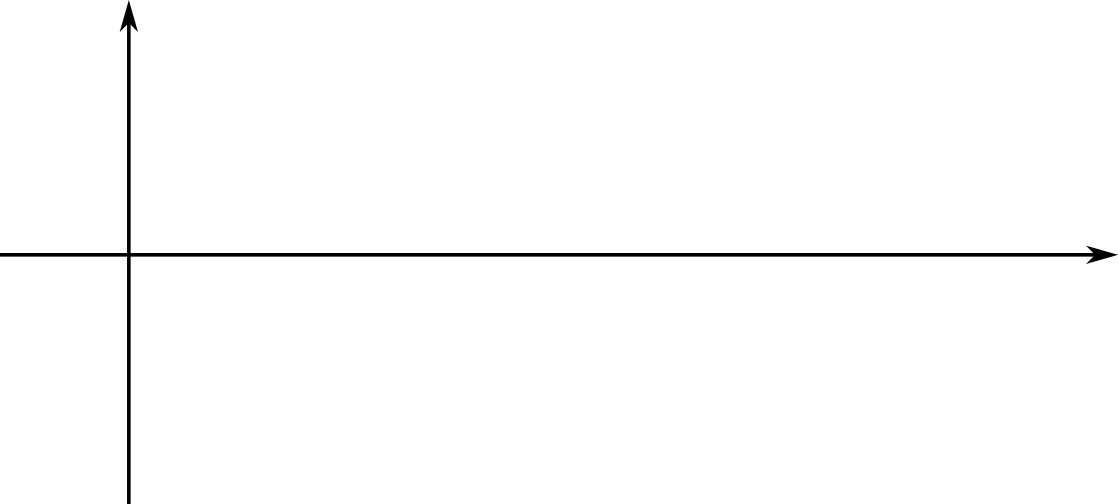
\includegraphics[scale=.40]{images/topic3_fig1.png}

				\btVFill
			\end{frame}

			\begin{frame}
				\frametitle{\sectionIIIsubsectionIItitle}
				\bigskip
				
				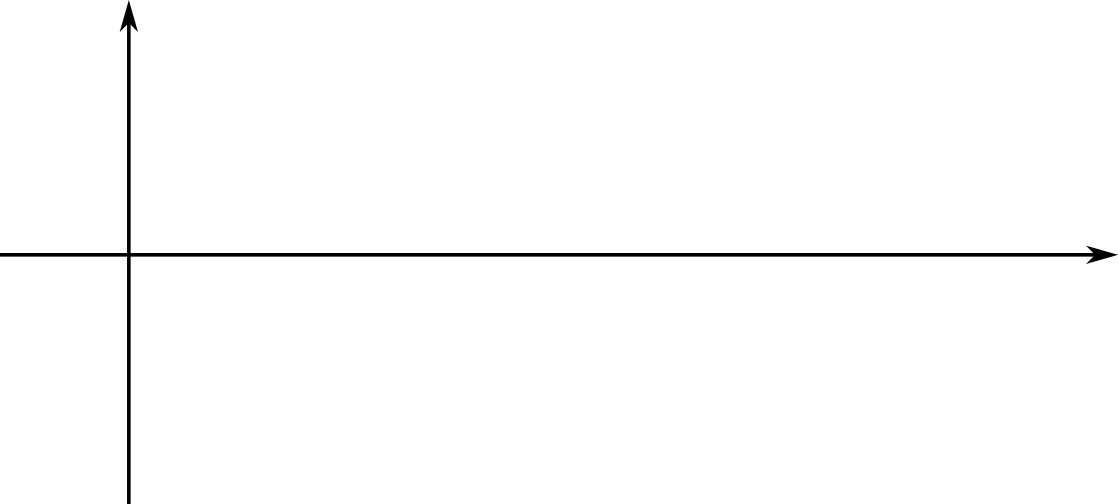
\includegraphics[scale=.40]{images/topic3_fig1.png}

				\btVFill
			\end{frame}

			\begin{frame}
				\frametitle{\sectionIIIsubsectionIItitle}
				\bigskip
					
				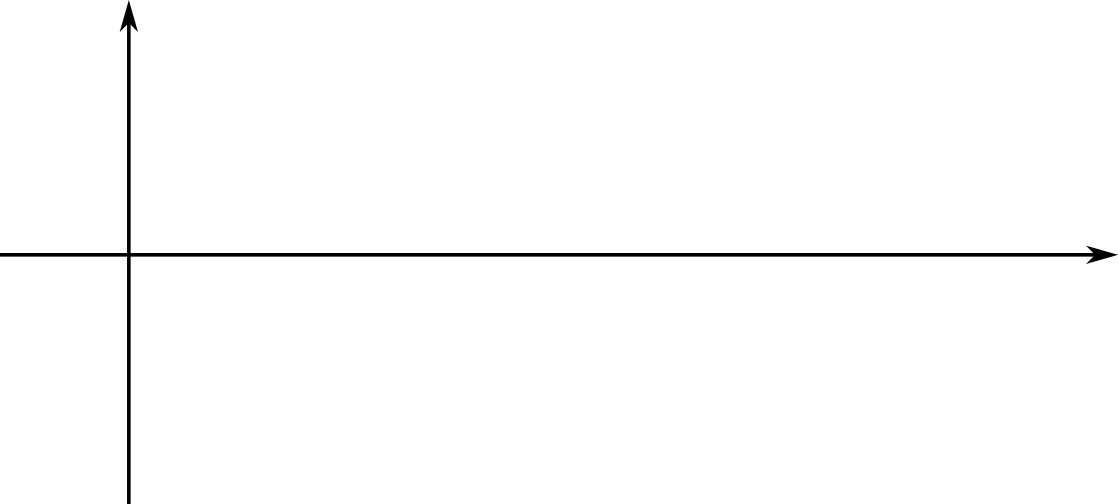
\includegraphics[scale=.40]{images/topic3_fig1.png}
				
				\btVFill
			\end{frame}

		% section III subsection III
		\subsection{\sectionIIIsubsectionIIItitle}\label{sectionIIIsubsectionIII}

			\begin{frame}
				\frametitle{\sectionIIIsubsectionIIItitle}
				\bigskip

				\begin{enumerate}
					\item \vspace{5mm}
					\item \vspace{5mm}
					\item \vspace{5mm}
					\item \vspace{5mm}
				\end{enumerate}
				
				\btVFill
			\end{frame}

			\begin{frame}
				\frametitle{\sectionIIIsubsectionIIItitle}
				\bigskip

				See MATLAB example.
 				
				\btVFill
			\end{frame}

			\begin{frame}
				\frametitle{\sectionIIIsubsectionIIItitle}
				\bigskip

				\textbf{General Use Algorithm:} the bisection method can also be used to solve the general root finding problem \vspcc
				\underline{Pros:}
				\begin{itemize}
			    	\item -
			    	\item -
			    	\item -
				\end{itemize} 

				\underline{Cons:}
				\begin{itemize}
					\item -
					\item -
					\item -
				\end{itemize}
				
				\btVFill
			\end{frame}



	% Section IV
	\section{\sectionIVtitle}\label{sectionIV}

		% section IV Outline
		\begin{frame}
			\large \textbf{Topic 3 - \sectionIVtitle} \vspace{3mm}\\

			\begin{itemize}
				\item \hyperlink{sectionIVsubsectionI}{\sectionIVsubsectionItitle} \vspc %  section IV subsection I
				\item \hyperlink{sectionIVsubsectionII}{\sectionIVsubsectionIItitle} \vspc % section IV subsection II
				\item \hyperlink{sectionIVsubsectionIII}{\sectionIVsubsectionIIItitle} \vspc % section IV subsection III
				\item \hyperlink{sectionIVsubsectionIV}{\sectionIVsubsectionIVtitle} \vspc % section IV subsection IV
			\end{itemize}

		\end{frame}

		% section IV subsection I
		\subsection{\sectionIVsubsectionItitle}\label{sectionIVsubsectionI}

			\begin{frame}
				\frametitle{\sectionIVsubsectionItitle}
				\bigskip

				\textbf{A Mechanical Design Problem}\\	
		
				As an engineer you are asked to design a structure. The geometry of this structures is simple but certain properties are critical. Also you want to spend as little as possible on materials.
					
				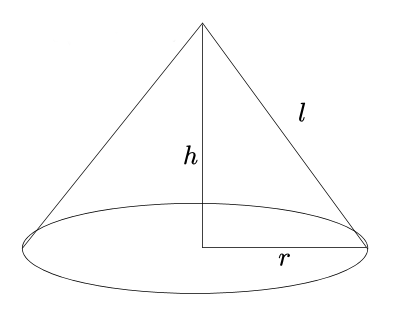
\includegraphics[scale=.35]{images/lecture3_fig1.png}\\
					
				You are required to design is a cone with a surface area of exactly $25 m^2$ to a tolerance of 0.1 $m^2$ and a height of exactly $1 m$. Your goal is to find the radius in meters.\\
						
				\btVFill
			\end{frame}

			\begin{frame}
				\frametitle{\sectionIVsubsectionItitle}
				\bigskip

				What is the {\it mathematical model} of the cone?  

				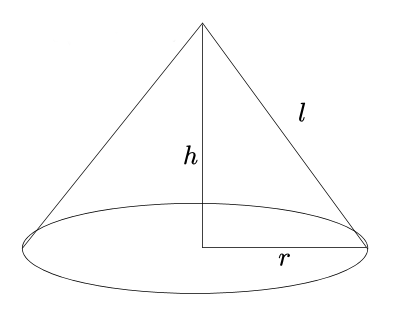
\includegraphics[scale=.35]{images/lecture3_fig1.png}\\
				\scalebox{1.2}{surface area, $s=\pi r l = \pi r \sqrt{h^2+r^2}$} \\
				\scalebox{1.2}{volume, $v=\pi r^2 \frac{h}{3}$} \\

				\btVFill
			\end{frame}

		% section IV subsection II
		\subsection{\sectionIVsubsectionIItitle}\label{sectionIVsubsectionII}

			\begin{frame}
				\frametitle{\sectionIVsubsectionItitle}
				\bigskip

				How are you going to solve this problem?
				\vspace{50mm}	

				\btVFill
			\end{frame}

			\begin{frame}
				\frametitle{\sectionIVsubsectionItitle}
				\bigskip

				How are \underline{you} going to {\it design} the cone? \vspace{5mm}\\
				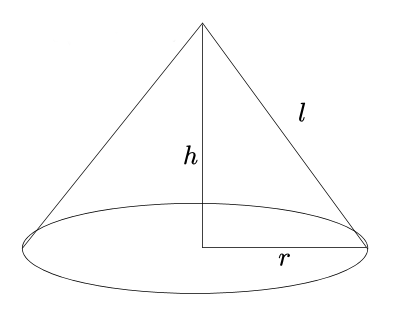
\includegraphics[scale=.35]{images/lecture3_fig1.png}\\

				\btVFill
			\end{frame}	


\end{document}





